\chapter{Implementation}
As far as code implementation goes, the aforementioned algorithms all share the following structure:
\begin{verbatim}
void step(){
    sample_allocations();
    sample_unique_values();
}

void run(){
    initialize();
    unsigned int iter = 0;
    while(iter < maxiter){
        step();
        if(iter >= burnin){
            save_iteration(iter);
        }
        iter++;
    }
}
\end{verbatim}
In particular, the blocked Gibbs algorithm has an additional phase in \verb|step()|, \verb|sample_weights()|. Moreover, as discussed in chapter \ref{algo}, all the algorithms can be generalized including further Gibbs sampling steps to update the hyperparameters of $G_0$ or the total mass parameter $M$.
Each implemented algorithm will be discussed in detail in its own section.
As for the general structure of an algorithm class, a template approach was chosen, to allow the use of several layers of complexity based on the needs of the user:
\begin{verbatim}
template<template <class> class Hierarchy, class Hypers,
         class Mixture> class Algorithm
\end{verbatim}
That is, \verb|Hierarchy<>|, \verb|Hypers|, and \verb|Mixture| are not actual implemented classes, but rather proxy names for classes which will be received as \emph{parameters} by the algorithm class.
These classes must have a \emph{common interface} in order for them to be passed as parameters, as explained in the following section.
An example with actual class names, as found in the \verb|main.cpp| file, is:
\begin{verbatim}
Neal8<NNIGHierarchy, HypersFixed, SimpleMixture> sampler8;
\end{verbatim}
As a final introductory note, probability distributions and random sampling were handled through the \verb|Stan| library, whilst the popular \verb|Eigen| library was exploited for the creation of the necessary matrix-like objects and the use of matrix-algebraic operations throughout the code.

\section{Auxiliary classes}
First of all, we must briefly describe the auxiliary classes that are used as parameters for the algorithms:
\begin{itemize}
	\item The \verb|Mixture| classes contain all information about the mixing part of the DPM model, namely the total mass parameter and its prior distribution, if any.
	We implemented the \verb|SimpleMixture| class, which represents a fixed total mass parameter without any prior on it, and contains the \verb|totalmass| member as well as a getter and a setter (\verb|get_totalmass()|, \verb|set_totalmass()|).
	\item The \verb|Hypers| classes contain all information about the hyperparameters of the hierarchy, including their values (if fixed) or their prior distributions (if not).
	We implemented the \verb|HypersFixedNNIG| class, which contains the four fixed parameters \verb|mu0|, \verb|lambda|, \verb|alpha0|, and \verb|beta0| of the Normal-NIG hierarchical model, and their respective getters and setters.
	\item The \verb|Hierarchy<Hypers>| classes are template classes themselves and accept any \verb|Hypers| class as template parameter.
	A \verb|Hierarchy<>| class contains a vector \verb|state| which stores the current values of the likelihood parameters, as well as a pointer to a \verb|Hypers| object -- this is why \verb|Hypers| is required as a parameter for \verb|Hierarchy<>|.
	A pointer is chosen instead of an actual object, since multiple \verb|Hierarchy<>| objects will be created and stored by the algorithms; the \verb|state|s of these objects will of course share the same prior, and with a pointer to \verb|Hypers| the updating of the prior will only happen once rather than one time per object.
	A \verb|Hierarchy<>| class also contains functions to:
	\begin{itemize}
		\item evaluate the marginal distribution (provided it is known in closed form) and the log-likelihood in a given set of points, given the current \verb|state|;
		\item compute the posterior parameters with respect to a given set of observations;
		\item generate new values for the \verb|state| both according to its prior and to its posterior distribution;
		\item get and set class members, as with the other classes.
	\end{itemize}
	In particular, we implemented the \verb|HierarchyNNIG| class, which represents the Normal-NIG model described in section \ref{nnig}.
	The \verb|state| holds the values for $\boldsymbol\phi = (\mu,\sigma)$.
\end{itemize}
Any class representing any type of hierarchy or parameters can be built as long as it possesses the above interface, which is required for their use in the implemented algorithms. \\
We will be now first examining the \verb|Neal8| class as an example.

\section{\texttt{Neal8} algorithm}
Relying on the algorithm described in section \ref{neal8}, we proceed to describe our implementation of it.
Aside from the usual getters and setters, as well as constructors, the \verb|Neal8| class contains the following members:
\begin{verbatim}
unsigned int n_aux;
unsigned int maxiter;
unsigned int burnin;
unsigned int num_clusters;
std::mt19937 rng; // random number generating engine
\end{verbatim}
These are the parameters of the method, and are rather self-explanatory.
Their values are initialized either via the constructors or the setters.
If \verb|num_clusters| is not provided, it will be automatically set equal to the number of data points, thus starting the algorithm with one datum per cluster. \\
The data and values containers were implemented as follows:
\begin{verbatim}
std::vector<double> data;
std::vector<unsigned int> allocations;
std::vector<Hierarchy<Hypers>> unique_values;
std::vector<Hierarchy<Hypers>> aux_unique_values;
Mixture mixture;
\end{verbatim}
The algorithm will keep track of the labels representing assignments to clusters via the \verb|allocations| vector.
For instance, if one has \verb|allocations[5] = 2|, it means that datum number 5 is associated to cluster number 2.
Note that indexing for both data and clusters starts at zero, so this actually means that we have the sixth datum being assigned to the third cluster. \\
The containers for the unique values $\boldsymbol\phi$ hold objects of type \verb|Hierarchy<>| because each $\boldsymbol\phi$ is associated to a cluster, which is in fact a small hierarchy that can have its own hyperprior in the general case.
The same reasoning goes for \verb|aux_unique_values|, the $m$ auxiliary blocks, from which the algorithm may draw in order to generate new clusters. \\
As for the members used for running the algorithm:
\begin{verbatim}
void initialize();
void sample_allocations();
void sample_unique_values();
void step(){
    sample_allocations();
    sample_unique_values();
}
void save_iteration(unsigned int iter);
void run();
\end{verbatim}
Aside from \verb|run()|, whose code was shown at the beginning of this section, we shall briefly describe the implementation of these functions:
\begin{itemize}
	\item \verb|initialize()| creates \verb|num_clusters| clusters and randomly assigns each datum to one of them, while making sure that each cluster contains at least one.
	This assignment is done through changing \verb|allocations| components, as explained earlier.
	\item In \verb|sample_allocations()|, a loop is performed over all observations $i=1:n$.
	A vector \verb|card| is first filled, with \verb|card[j]| being the cardinality of cluster $j$.
	The algorithm mandates that \verb|data[i]| be moved to another cluster; thus, if the current cluster is a singleton, its $\boldsymbol\phi$ values are transferred to the first auxiliary block.
	Then, each auxiliary block (except the first one if the above case occurred) generates new $\boldsymbol\phi$ values via the hierarchy's \verb|draw()| function.
	Now a new cluster, that is, new $\boldsymbol\phi$ values, for \verb|data[i]| needs to be drawn.
	A vector \verb|probas| with \verb|n_unique+n_aux| components is filled with the probabilities of each $\boldsymbol\phi$ being extracted, in line with (\ref{neal8prob}).
	Computations involve, among other things, the \verb|card| vector, the likelihood \verb|like()| evaluated in \verb|data[i]|, and the total mass parameter.
	Then, the new value for \verb|allocations[i]| is randomly drawn according to the computed \verb|probas|.
	Finally, four different cases of updating \verb|unique_values| and \verb|card| are handled separately, depending on whether the old cluster was a singleton or not, and whether an auxiliary block or an already existing cluster was chosen as the new cluster for \verb|data[i]|.
	This is done because depending on the case, clusters are either unchanged, increased by one, decreased by one, or moved around.
	\item In \verb|sample_unique_values()|, for each cluster $j$, their $\boldsymbol\phi$ values are updated through the \verb|sample_given_data()| function, which takes as argument the vector \verb|curr_data| of data points which belong to cluster $j$.
	Since we only keep track of clusters via their labels in \verb|allocations|, we do not have a vector of actual data points stored for each cluster.
	Thus we must fill, before the loop on $j$, a matrix \verb|clust_idxs| whose column $k$ contains the index of data points belonging to cluster $k$.
	\verb|clust_idxs| is then used in the $j$ loop to fill \verb|curr_data| with the actual data points of cluster $j$.
	\item \verb|save_iteration| will be examined in the next section.
\end{itemize}

\section{\texttt{Neal2} algorithm}
The structure of the \verb|Neal2| class is similar to the one of \verb|Neal8| described above.
The only relevant differences are the obvious lack of \verb|aux_unique_values| and most of the \verb|sample_allocations()| phase.
As discussed in section \ref{neal2}, this algorithm exploits conjugacy, thus this function requires specifically implemented hierarchies, in which the marginal distribution of the data with respect to $\boldsymbol\theta$ is provided in closed form.
In our case, a Normal-NIG specialization for the \verb|Neal2| template class was implemented.
In \verb|sample_allocations()|, a loop is performed over observations $i$ and the \verb|card| vector is built, just as before.
The \verb|probas| vector of weights for the new allocation value is computed, according to the probabilities (\ref{probasneal2}), by also using the marginal density in \verb|data[i]|, which is known to be a Student's $t$ as mentioned in section \ref{nnig}.
After the new \verb|allocations[i]| is drawn according to \verb|probas|, four cases are handled separately as before, depending on whether the old cluster was a singleton and whether \verb|data[i]| is assigned to a new cluster.
Indeed, in such a case, a new $\boldsymbol\phi$ value for it must be generated, and this must be handled differently by the code if an old singleton cluster was just destroyed (as the new cluster must take its former place).





\part{Applications}

\chapter{Applications}
These algorithms can also be used for two useful practical purposes: \emph{cluster estimation} and \emph{density estimation}.
Both processes, however, require the whole chain to be saved, that is, at each iteration the current values of states and allocations must be stored in some data structure.
For this purpose, we used the Protocol Buffers library, which needs a short introduction. \\
Protocol Buffers, or \verb|protobuf| for short, was developed by Google and allows automatic generation of data-storing C++ classes by defining a class skeleton in a \verb|.proto| file.
This also allows easy interfacing with other programming languages such as R and Python. \\
We built our template as follows:
\begin{verbatim}
message UniqueValues {
    repeated double params = 1;
}
message IterationOutput {
    repeated int32 allocations = 1;
    repeated UniqueValues phi = 2;
}
message ChainOutput {
    repeated IterationOutput state = 1;
}
\end{verbatim}
Here \verb|message| and \verb|repeated| are the \verb|protobuf| equivalent of classes and vectors respectively, while the numbers 1 and 2 just act as identifiers for the fields in the messages.
After generating the corresponding C++ classes via the \verb|protoc| compiler, we were able to add the following members to the \verb|Neal8| and \verb|Neal2| classes:
\begin{verbatim}
ChainOutput chain;
IterationOutput best_clust;
std::pair< std::vector<double>, Eigen::VectorXd > density;
\end{verbatim}
For each iteration after the burn-in phase, the \verb|save_iteration()| function saves all state values of the current iteration into the \verb|chain| pseudo-vector in the appropriate structure.
On the other hand, \verb|best_clust| represents the state of a single iteration, and it is the object where the result of the clustering analysis will be saved.
The \verb|density| object shares a similar purpose for the density estimation part, albeit not actually generated via \verb|protobuf|.
It will be filled with a grid of points in which the density will be evaluated, and the evaluations of the density themselves. \\
We will be explaining in thorough detail these two useful applications in the next lines.

\section{Cluster estimation}
Suppose we wish to estimate the real clustering of the data, assuming the DPM model holds true.
A first rough estimate is the \emph{final clustering}, that is, the state values corresponding to the last iteration of the algorithm.
This estimate does not require an appropriate function to be implemented, since the state values are already available in \verb|allocations| and \verb|unique_values| after the algorithm is \verb|run()|.
However, due to the oscillating behavior of the clusters (as we shall see later on), the last clustering may not be the optimal one.
Instead, we chose to implement a \emph{least square} estimate in the following function:
\begin{verbatim}
unsigned int cluster_estimate();
\end{verbatim}
This function exploits the \verb|chain| pseudo-vector, in which states of all iterations of the algorithm were saved via \verb|save_iteration()| (of course, only after the burn-in phase) and the \verb|protobuf| library.
This function loops over all \verb|IterationOutput| objects in \verb|chain|, finds the iteration at which the best clustering occurred, saves the whole object into the \verb|best_clust| class member, and returns the iteration number of this best clustering.
As briefly touched upon earlier, the best clustering is found via the minimization of the squared posterior \emph{Binder's loss function}.
An equivalent approach (see \cite{beep} lecture on BNP clustering) is computing the so-called \emph{dissimilarity matrix} for each iteration, computing its sample mean over all iterations, and finding the iteration that is the closest to the mean with respect to the \emph{Frobenius norm}. 
More specifically, for each iteration $k$, the dissimilarity matrix $D^{(k)}$ is a symmetric, binary $n$-by-$n$ matrix (where $n$ is the number of available observations) whose entries $D^{(k)}_{ij}$ are $1$ if datum $i$ and $j$ are placed in the same cluster at iteration $k$ and $0$ otherwise.
After each $D^{(k)}$ and the sample mean $\bar{D} = \frac{1}{K} \sum_k D^{(k)}$ are computed, where $K$ is the number of iterations (not counting the ones in the burn-in phase), the best clustering $\hat{k}$ is found by minimizing the Frobenius norm of the difference with $\bar{D}$:
$$
\hat{k} = \argmin_k \left\lVert D^{(k)} - \bar D \right\rVert_F^2 = \argmin_k \sum_{i,j} \left( D^{(k)}_{ij} - \bar{D}_{ij} \right)^2.
$$
By virtue of the involved matrices being symmetric, the latter summation can be computed over all $i<j$ instead of all $i,j$ for efficiency. \\
The convergence in mean of the algorithm grants the correctness of this least square estimate, at it is the closest available approximation to the mean dissimilarity matrix.

\section{Density estimation} \label{dens-estim}
One other important application of clustering algorithms is the estimation of the density according to which the data points are distributed.
This is done differently in both the \verb|Neal2| and \verb|Neal8| algorithms, as the former can exploit the conjugacy of the hierarchical model.
In either case, the following function was implemented:
\begin{verbatim}
void eval_density(const std::vector<double> grid);
\end{verbatim}
It accepts a grid of points in which the density will be evaluated.
This grid is stored in the \verb|density| member object, as well as the computed evaluations themselves in form of a vector from the \verb|Eigen| library.
Just like for the cluster estimate, the computation will access all iterations stored in the \verb|chain| pseudo-vector.
In both \verb|Neal8| and \verb|Neal2|, a loop is performed over the iterations $k$.
Suppose this iterations has $J$ clusters, that is, $j=0:J-1$.
The \verb|card| vector is once again computed, where $\texttt{card[j]} = n^{(k)}_j$ is the cardinality of cluster $j$.
Then, for each point $x$ in \verb|grid|, we compute the local estimate of the density, that is, only taking iteration $k$ into account:
\begin{equation}\label{localdens}
	\begin{aligned}
	\hat f^{(k)}(x) \ = \ \sum_j \frac{n^{(k)}_j}{M+n} f\left(x | \boldsymbol{\phi}^{(k)}_j\right) \ + \ \frac{M}{M+n} m(x)
	\end{aligned}
\end{equation}
That is, the local estimate is a weighted mean of the likelihood given the unique values $\boldsymbol{\phi}^{(k)}_j$ of cluster $j$ and the marginal distribution $m(x)$, taken from the appropriate function in the \verb|Hierarchy<>| class.
The weights of the clusters are proportional to their size $n^{(k)}_j$, while the ``virtual'' cluster of the marginal counts as having size $M$, the total mass parameter ($n$ is the total number of observations, as per usual).
The marginal distribution is only known under the conjugacy assumption in the \verb|Neal2| algorithm.
In particular, for a Normal-NIG model $m(x)$ is a Student's $t$ as explained in section \ref{nnig}.
In the \verb|Neal8| algorithm, $m(x)$ is not available in closed form, and thus it is replaced in the above formula by the following approximation:
\begin{equation}\label{margneal8}
	\begin{aligned}
		\hat m(x) = \frac{1}{m} \sum_{h=0}^{m-1}  f\left(x | \boldsymbol{\phi}_h\right)
	\end{aligned}
\end{equation}
where we use $m$ unique values, that is, one for each of the $m = \verb|n_aux|$ auxiliary blocks of the algorithm, drawn from the base measure: $\boldsymbol{\phi}_{h} \overset{\text{iid}}{\sim} G_0, \ h=0:m-1$. \\
Finally, the \emph{empirical density} is computed as the mean over all $K$ iterations:
$$
\hat f(x) = \frac{1}{K} \sum_k \hat f^{(k)}(x)
$$
and saved into the \verb|density| object.
Again, this estimate approaches the true posterior density of the data thanks to the convergence in mean of the chain.

\section{Saving estimates to files}
We also implemented the following functions in each \verb|Algorithm| class, which save data from the class into text files in order to ease exportation to other programs or computers:
\begin{verbatim}
const void write_final_clustering_to_file(
           std::string filename = "final_clust.csv");
const void write_best_clustering_to_file(
           std::string filename = "best_clust.csv");
const void write_chain_to_file(
           std::string filename = "chain.csv");
const void write_density_to_file(
           std::string filename = "density.csv");
\end{verbatim}
They can be called as need be from the \verb|main.cpp| file.
If a file name is not provided, the above default names will be used.
The former two create a \verb|.csv| file with the columns being, in order, data index, data value, allocation, unique values (one per column).
\verb|write_chain_to_file()| has the same columns as the previous functions, but adds one more column containing the iteration number (starting from $0$) as the first one.
Finally, \verb|write_density_to_file()| has values of $x$ in the first column and the corresponding $\hat f(x)$ in the second one.


\chapter{Results}
Our clustering analysis was conducted on $n=100$ observations, the former 50 of which were iid sampled from a $\Nc(4,1)$ and the latter from a $\Nc(7,1)$, which were saved in the \verb|data.csv| file.
We chose the prior parameters for the Normal-NIG model (\ref{nnig}) as follows: $\mu_0 = 5, \lambda_0 = 1, \alpha_0 = 2, \beta_0 = 2$.
The \verb|Neal8| algorithm with $m=3$ auxiliary blocks was run for 20000 iterations, and the first 5000 were discarded as burn-in, for a total of $K=15000$ valid iterations.
We will keep these parameters values fixed unless explicitly stated. \\
The following test data were all saved to \verb|.csv| files and used for the realization of plots with the \verb|ggplot2| R package.
All scripts and data sheets are available in the GitHub repository of our library.

\section{Oscillations}
After running the algorithm as described above with total mass $M=0.25$, we find that the obtained best clusterings (again, in the lest square sense) and local density estimates are highly fluctuating over the iterations of the algorithm:
\begin{figure}[h]
	\centering
	\begin{minipage}{0.5\textwidth}
		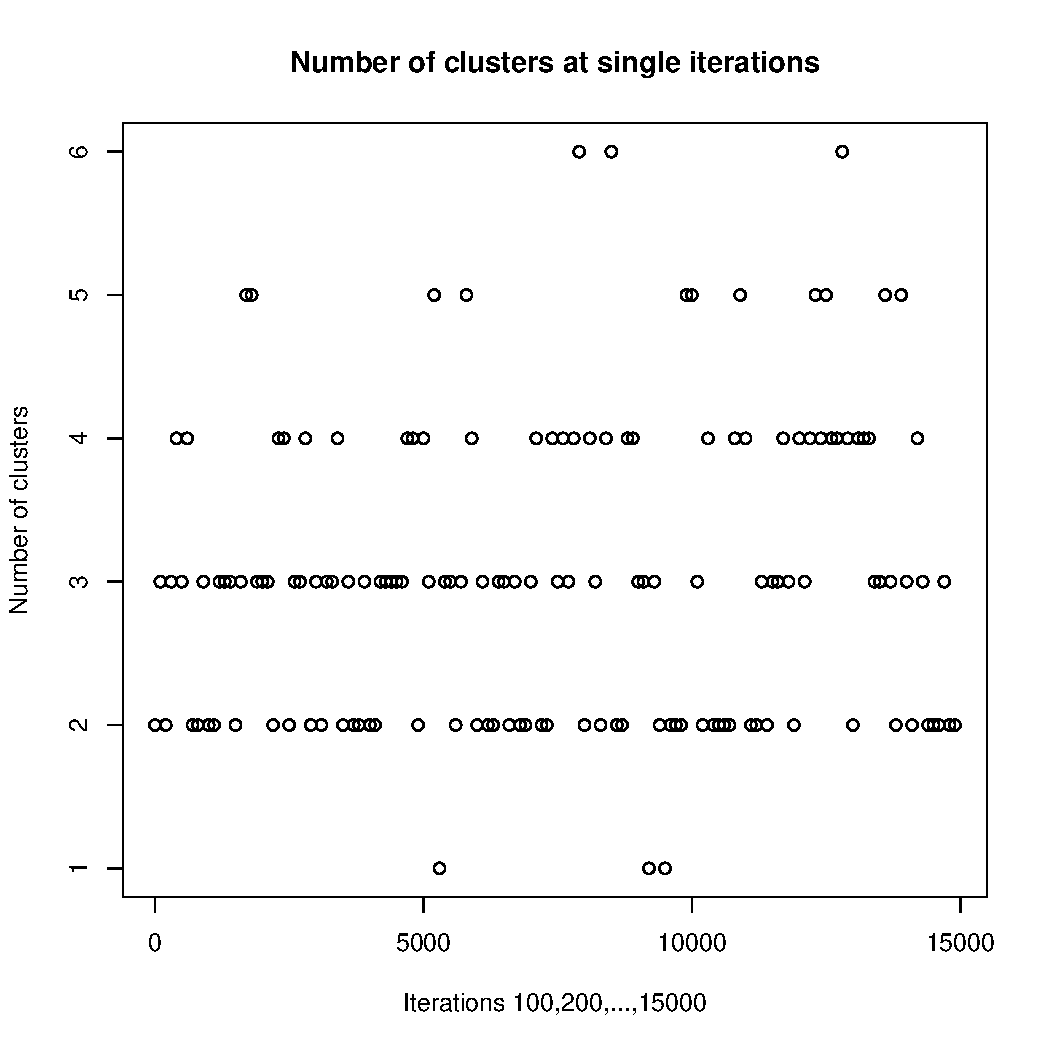
\includegraphics[scale=0.35]{etc/cardinalities_thinned.pdf}
	\end{minipage}%
	\begin{minipage}{0.5\textwidth}
		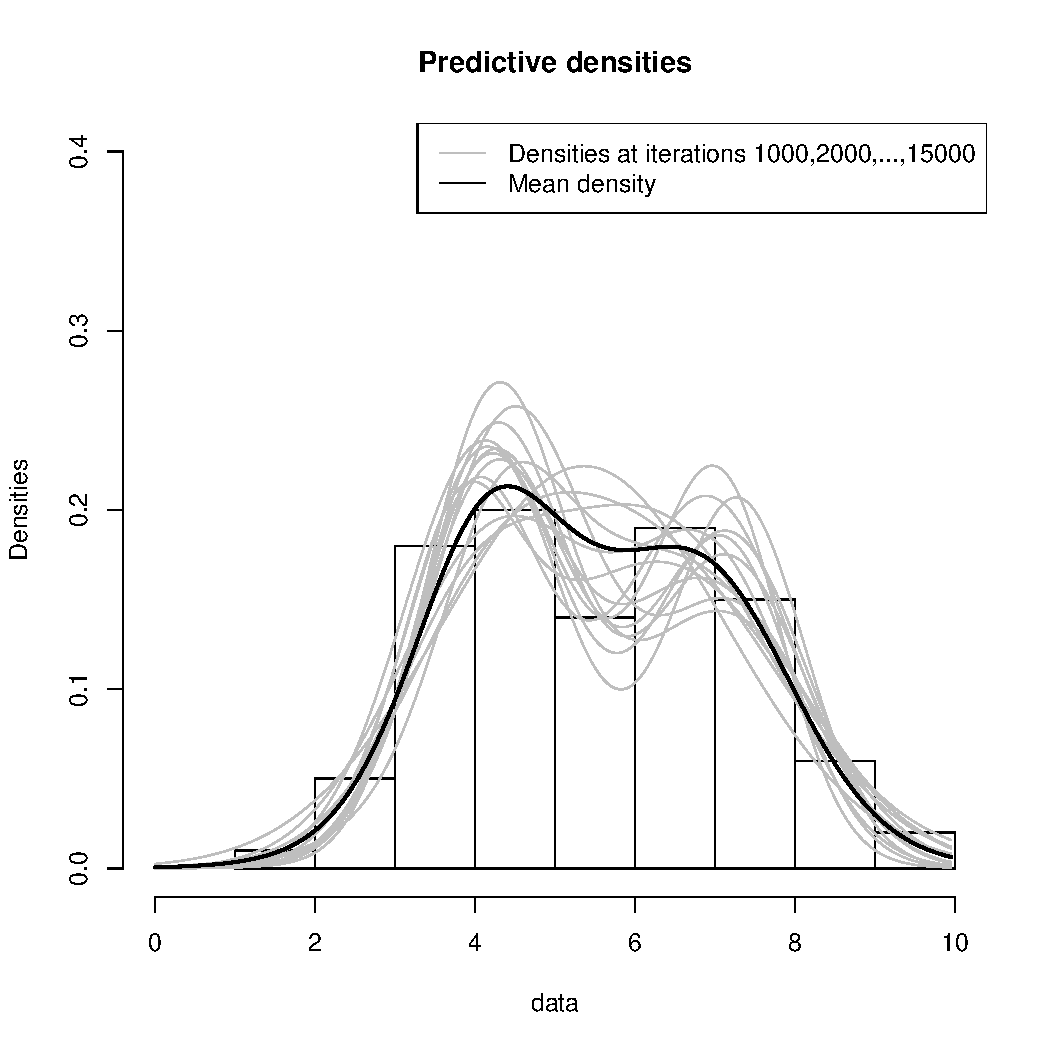
\includegraphics[scale=0.35]{etc/densities_iters.pdf}
	\end{minipage}
\end{figure}

In both plots, a thinning of one iteration every 100 and every 2500, respectively, was performed for better readability of the plot.
In the right side plot, the local densities are compared with the histogram of the data as well as the final estimate provided by the mean density.
We can see that the number of clusters at all iterations varies significantly between 1 and 6, even in the last thousands of iterations, and the same behavior applies to the local density estimates. 
This is further confirmation of the fact that the single iterations themselves do not converge.
Instead, as previously discussed, the convergence is in the \emph{mean}, both for the density estimate and for the average dissimilarity matrix which we use to find the best clustering.

\section{Total mass}
Let us now examine the role of the total mass parameter, $M$.
We ran the algorithm with several values for $M$ whilst keeping the other parameters unchanged from the ones indicated at the beginning of the section.
For each $M$, we saved the number of clusters of the best clustering produced by the algorithm, and plotted it against the corresponding $M$:

\begin{figure}[h]
	\centering
	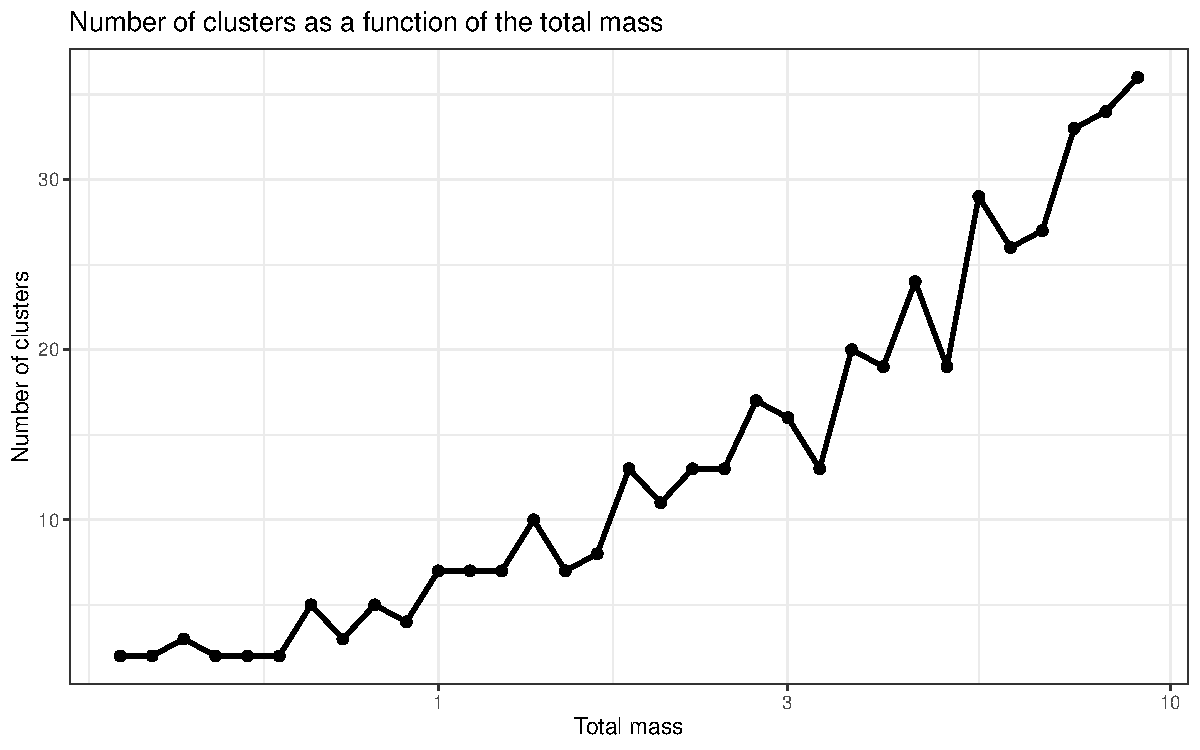
\includegraphics[scale=0.6]{etc/num_clust_M.pdf}
\end{figure}

Note that the values for $M$ were chosen so as to be evenly spaced in log-scale, thus the abscissa is in log-scale as well.
We can note that the clusters are increasing with the total mass.
This is consistent with the fact that the probability of creating a new cluster is proportional to $M$, as seen in (\ref{neal8prob}). \\
Moreover, the density estimates for some of the values of $M$ (again, compared with the histogram of the data) are as follows:

\clearpage

\begin{figure}[h]
	\centering
	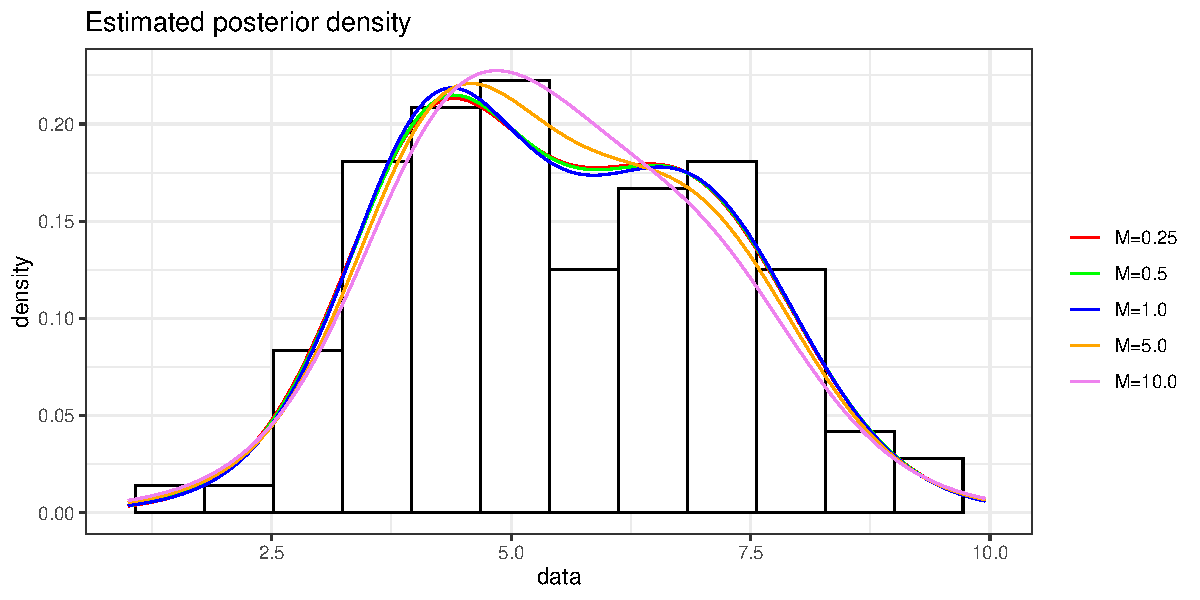
\includegraphics[scale=0.6]{etc/dens_withMm3.pdf}
\end{figure}


In our case, lower values for the total mass account better for the distribution of the data points, with the modes being near the real expected values of the two normal distributions, 4 and 7.
On the other hand, higher values tend to clump together all 100 observations as though they were extracted from a single distribution.
As we can see, the total mass $M$ acts as smoothing parameter and, given its strong influence on the number of mixture components, it is a prime candidate for a prior distribution being put onto it.



\section{Auxiliary blocks}
We shall now try and change the number of auxiliary blocks $m$, and check how this impacts the density estimation.
For this test, a large total mass $M=10$ was chosen; the reason being that a small $M$ would not allow significant differences as $m$ changes.
Indeed, $m$ directly influences only the estimate (\ref{margneal8}) of the marginal distribution, that has a weight of $\frac{M}{M+n}$ (as seen in (\ref{localdens})), which is negligible if $M$ is small.
Therefore, $M=10$ was picked, and the result was the following:


\begin{figure}[h]
	\centering
	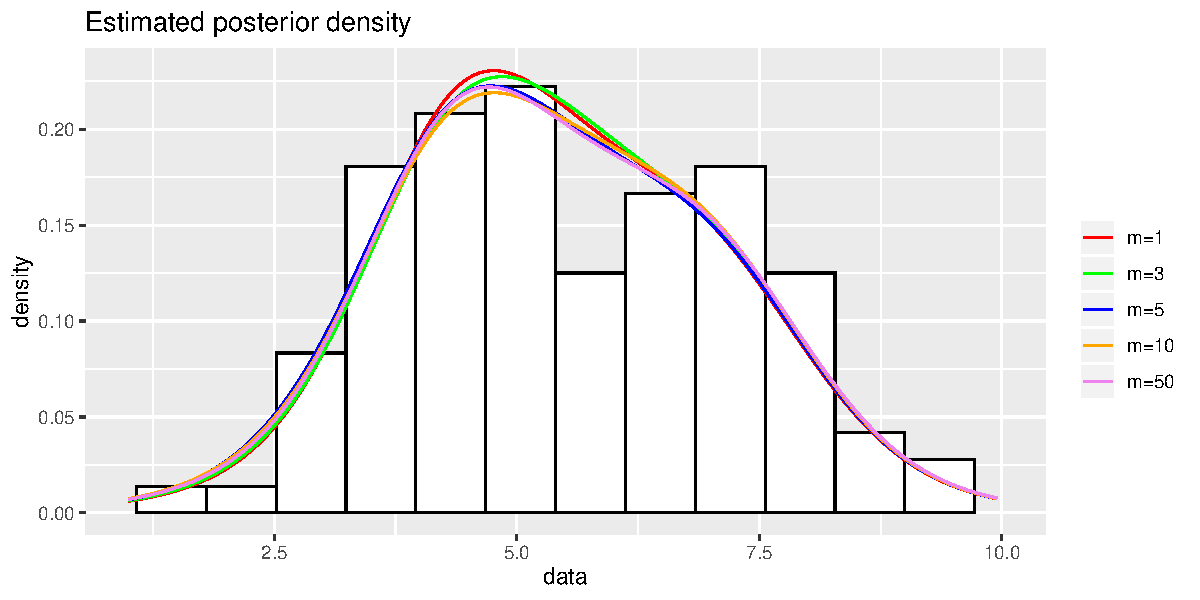
\includegraphics[scale=0.6]{etc/dens_withmM10.pdf}
\end{figure}

Note that a larger $m$ gives a better estimate of the marginal, because the sample mean is computed over a larger number of terms and the algorithm approximates the behavior of the algorithm \verb|Neal2|.



\section{Density components}
We now wish to visualize how the local density is computed at a given sample iteration.
Let us run again the \verb|Neal8| algorithm with both $M=0.25$ and $m=3$ fixed, and then use the \verb|cluster_estimate()| function to extract the best clustering for the data.
We find that it is at iteration 2490, which gives 2 clusters.
As shown in \ref{localdens}, each of these clusters has its own density estimate, which we refer to as \emph{component}, and a weight attached to it proportional to its cardinality.
The weighted sum of these components gives the ``full'' local estimate of the density for that iteration.
This plot shows both the \emph{weighted} components and their sum:
\begin{figure}[h]
	\centering
	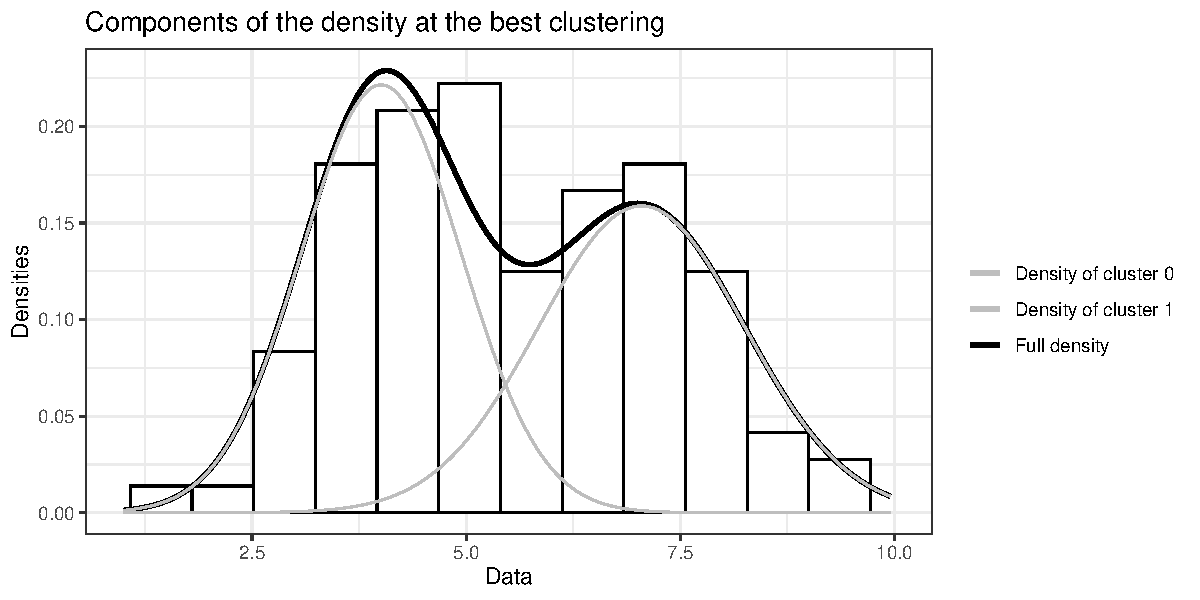
\includegraphics[scale=0.7]{etc/componentsM025m3_best.pdf}
\end{figure}

In this case the weights turn out to be approximately equal (0.52 and 0.48 respectively).
Again, the two components are concentrated around the true means (4 and 7) of the likelihoods of the data points, as expected. \\
In other cases, the best clustering may produce more than 2 clusters.
One such example is given by the best clustering of \verb|Neal8| run with $M=1$ (and $m=3$ as before), found at iteration 6611.
Although there are 7 clusters, all weights bar the first two are insignificant, making the corresponding components have almost zero impact in the weighted sum of the local estimate:

\clearpage

\begin{figure}[h]
	\centering
	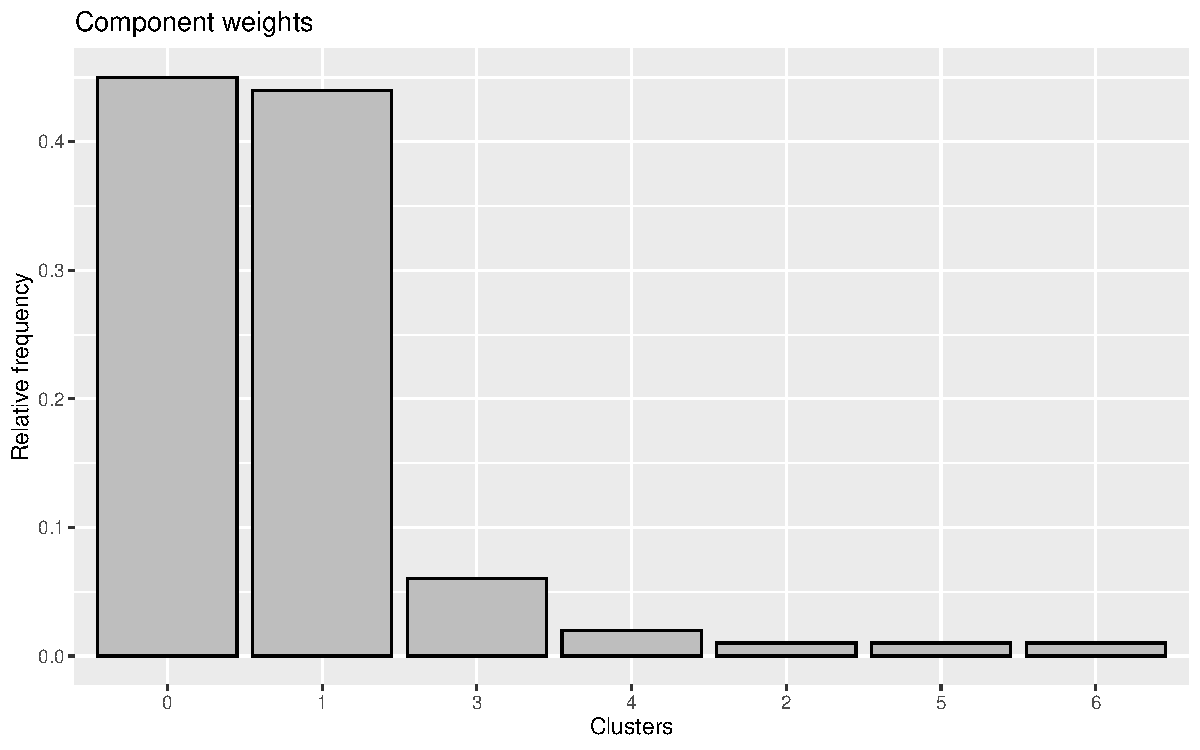
\includegraphics[scale=0.5]{etc/barplotM1m3.pdf}
\end{figure}



\section{\texttt{Neal2} vs \texttt{Neal8}}
Finally, we ran the \verb|Neal2| algorithm with the same parameters as \verb|Neal8| (indicated at the beginning of the section) as well as $M=10$ for both.
Again, a rather large total mass was chosen in order to better highlight the difference in the marginal estimate.
In fact, in the \verb|Neal2| case, since the marginal distribution is known in closed form, the estimate is more accurate:

\begin{figure}[h]
	\centering
	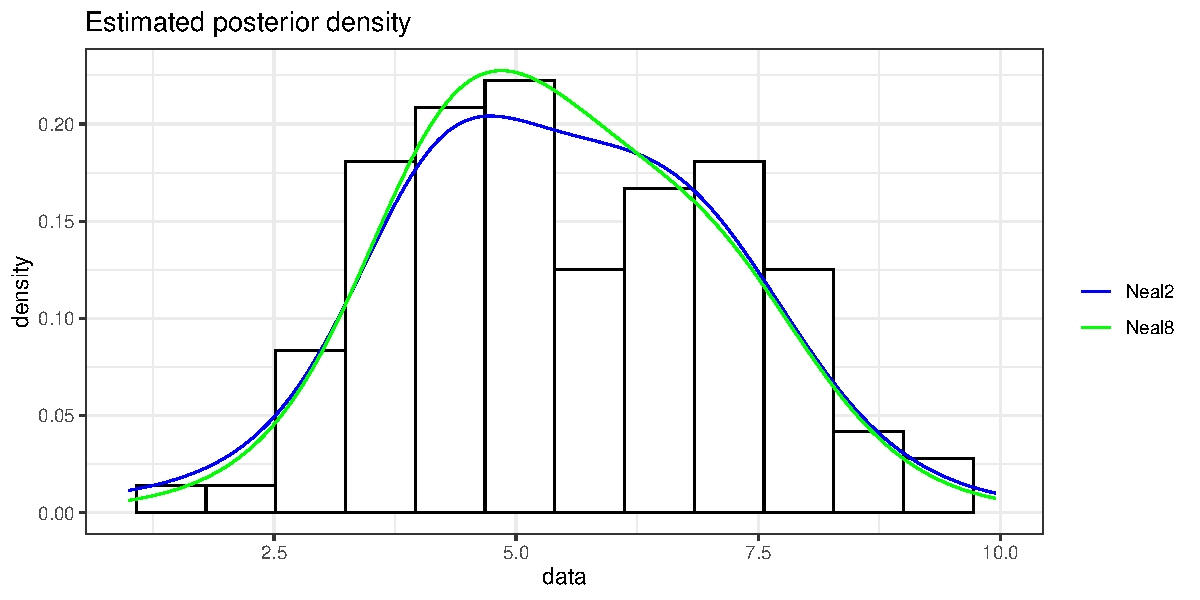
\includegraphics[scale=0.7]{etc/neal2_M10.pdf}
\end{figure}

\chapter{Extensions}
The \verb|bnplib| library has several possible extensions:
\begin{itemize}
	\item New types of \verb|Hypers| classes can be implemented, for example ones containing hyper-priors for some of the parameters if the model.
	The algorithm must be modified accordingly, for instance by adding extra steps (which are skipped if the hyperparameters are fixed).
	Changes depend on the type of parameter for which a prior is used; for example, a prior on the total mass parameter involves different steps than a prior on the parameters of the base measure.
	For a general outline of the necessary changes, see \cite{neal} section 7.
	\item Hierarchies other than the Normal-NIG can be created.
	This is enough to run \verb|Neal8| and \verb|Neal2| by passing the class name as parameter, provided that the \verb|Hierarchy| class has the appropriate interface.
	\item Interfaces with both R and Python can be easily implemented, thanks to the data structures provided by \verb|protobuf| and the already-available libraries \verb|Rcpp| and \verb|pybind| respectively.
	\item Algorithms can be re-adapted for the use of other mixture models, such as the Pitman-Yor process.
	\item Conjugacy-dependent algorithms such as \verb|Neal2| can be re-adapted to account for non-conjugacy, for example by using an Hamiltonian Monte Carlo sampler.
	\item Finally, a \emph{full generalization} of the library might be possible.
	That is, given the distributions of the likelihood, hyperparameters, etc, one might want an algorithm that works for the chosen specific model without needing and explicit implementation for it.
	This means, among other things, that one has to handle non-conjugacy for the general case.
	The main issue is that Stan distribution functions do not accept vectors of parameter values as arguments; thus, the updated values for distributions must be explicitly enumerated and given as arguments one by one to the Stan function.
	This requires to know in advance the number of parameters for all such distributions, which is impossible in the general case.
	Some advanced C++ techniques may be used to circumvent this hindrance, such as argument unpackers that transform a vector into a list of function arguments, and variadic templates, which are templates that accept any number of arguments.
	Theoretically, the latter would also allow the use of priors on the parameters of the hyper-prior itself, and so on, adding layers of uncertainty ad libitum.
	Although it is a hard task, we do think it is possible to achieve with reasonable effort.
\end{itemize}
